\apendice{Documentación de usuario}

\section{Introducción}
En esta sección se detallan los requerimientos de la aplicación, su instalación y despliegue (en el caso de \texttt{UBUMLaaS}) y se acompañan de una serie de indicaciones y consejos para su correcto uso.

De igual manera que en el Manual del Programador cada parte del proyecto, \texttt{IS-SSL} y \texttt{UBUMLaaS}, se describirá por su propio lado, de tal manera que aunque haya aspectos comunes, cada una su propia documentación de usuario.

\section{UBUMLaaS}
En esta sección se va a presentar el manual de usuario para el correcto uso de la plataforma \texttt{UBUMLaaS}, de tal forma que sirva como guía para comprender y consiguientemente poder utilizar eficientemente el \textit{software} desarrollado.
\subsection{Requisitos de usuarios}
Los requisitos mínimos para poder hacer uso de \texttt{UBUMLaaS} son:
\begin{itemize}
\item Disponer de una conexión a Internet.
\item Hacer uso de navegador web con soporte a HTML5.
\item Tener habilitado JavaScript en el navegador.
\item Tener una cuenta en la plataforma.
\end{itemize}
\subsection{Instalación}
Al tratarse de un producto web no se requiere de ningún tipo de instalación. Los navegadores Google Chrome, Mozilla Firefox, Safari y Microsfot Edge son soportados\footnote{Todos ellos han sido probados por el equipo de desarrollo y usuarios encuestados a  los que se les proporcionó un documento de uso básico y lo usaron en sus dispositivos cotidianos.}, siempre y cuando se encuentren en versiones compatibles con HTML5 y tengan activado el uso de JavaScript.

Independientemente del dispositivo de uso (ordenador de sobremesa, portátil, tableta o móvil), se requiere de conexión a Internet como es lógico. Pero no necesita de permisos adicionales, ha sido desarrollada de tal manera que utiliza la sesión local del navegador sin necesidad del uso de \textit{cookies}.

Aunque se hizo un intento de traducción a los lenguajes más comunes, finalmente se encuentra en inglés de forma única.

\subsection{Manual del usuario}
En esta sección se describe como un usuario nuevo puede registrarse en la aplicación desarrollada, iniciar sesión, crear sus propios experimentos, así como predecir nuevas etiquetas con modelos ya entrenados.

\subsubsection{Registro}

Lo primero de todo una vez se conozca la URL en la que se encuentra desplegada la aplicación, es acceder a la misma, y se llegará a una página web similar a la Figura~\ref{fig:index-no-login}, pudiendo variar en función de la resolución del dispositivo (dispositivos móviles no son recomendados pero si tabletas). 

\imagenFlotante{../img/anexos/manual-usuario/UBUMLaaS/index-no-login}{Página de inicio}{index-no-login}

Seguidamente se procederá a hacer \textit{click} en cualquiera de los dos botones \textit{Register} disponibles, en el centro de la pantalla o arriba a la derecha. Ambos redireccionarán al usuario a la página de registro, la cuál será igual a la Figura~\ref{fig:register}.

\imagenFlotante{../img/anexos/manual-usuario/UBUMLaaS/register}{Página de registro}{register}
Una vez el futuro usuario de la aplicación se encuentra en frente al formulario de registro deberá de cumplimentarlo teniendo en cuenta las siguientes restricciones:
\begin{itemize}
\item La dirección de correo electrónico será única en el sistema, además deberá de ser real y accesible pues a la que se mandará el correo electrónico de verificación de la cuenta.
\item El usuario deberá ser único en el sistema, en caso de ya existir, se le notificará cuando se registre, use su creatividad.
\item La contraseña deberá tener una longitud mínima de 8 caracteres, debiendo incluir al menos una letra mayúscula, una letra minúscula, un número y un carácter especial.
\item La confirmación de la contraseña implica que se debe repetir la contraseña ingresada anteriormente.
\item El país deberá ser seleccionado de la lista de países disponibles, encontrándose todos ellos en inglés, la búsqueda por teclado es soportada.
\item Se deberá indicar el uso que se le va a dar a la plataforma.
\end{itemize}

Finalmente una vez se pulse el botón \texttt{Register} el cliente recibirá un correo electrónico (revisar la carpeta de correo no deseado o SPAM) con el enlace de verificación de la cuenta que acaba de crear.

Es importante tener en cuenta que mientras la cuenta no se encuentre verificada, permanecerá inactiva. En caso de tener algún problema con la activación, se recomienda contactar con soporte desde el mismo correo electrónico con el que se registró para solucionar los problemas que hayan podido surgir.

\subsubsection{Iniciar sesión}
El proceso de inicio de sesión es tan directo como hacer \textit{click} en cualquiera de los botones dedicados a ello en el índice principal, ver Figura~\ref{fig:index-no-login}, y será redireccionado a la página de inicio de sesión, siendo esta última igual a la Figura~\ref{fig:login}. Seguidamente se deberán introducir las credenciales con las que el usuario se registró y tendrá acceso al sistema.

\imagenFlotante{../img/anexos/manual-usuario/UBUMLaaS/login}{Página de inicio de sesión}{login}

\subsubsection{Recuperar contraseña}
En caso de que el usuario necesite recuperar su contraseña, en la página de inicio de sesión, Figura~\ref{fig:login}, puede hacer \textit{click} en \textit{Forgot your password?}, en donde se redirigirá a la página de recuperación de contraseña, igual a la Figura~\ref{fig:recover-passwd}. 

Introduciendo el correo electrónico y se le enviará un enlace al mismo para reestablecerla.

\imagenFlotante{../img/anexos/manual-usuario/UBUMLaaS/recover-passwd}{Página de recuperar contraseña}{recover-passwd}

\subsubsection{Crear un nuevo experimento}
La funcionalidad principal proporcionada por \texttt{UBUMLaaS} es la de crear experimentos de \texttt{ML}, para ello una vez se inicia sesión se llega al índice de la plataforma, tal y como aparece en la Figura~\ref{fig:index-login}. Para llegar a la vista de crear un nuevo experimento se debe de hacer \textit{click} o en el botón en mitad de la pantalla que indica \textit{Create a new experiment}, o en la parte superior derecha, en el botón \textit{New Experiment}. Cualquiera de los dos botones redirigirá al usuario a la vista deseada.

\imagenFlotante{../img/anexos/manual-usuario/UBUMLaaS/index-login}{Índice principal de \texttt{UBUMLaaS}}{index-login}
\imagenFlotante{../img/anexos/manual-usuario/UBUMLaaS/create-experiment}{Vista de crear experimento}{create-experiment}

Llegando a una página similar a la Figura~\ref{fig:create-experiment} (la figura se encuentra con zoom al 90\% para poder visualizar toda la página). 

En este momento el usuario podrá rellenar todos los campos del formulario para crear su experimento deseado. Se recomienda rellenar los campos en el siguiente orden:
\begin{enumerate}
\item Seleccionar le conjunto de datos a utilizar, pudiendo en este momento subir uno propio a la plataforma. Los nombres de los conjuntos de datos no son modificables luego asegúrese de que es correcto. En caso de subir uno propio la página se auto-actualizará en el momento en el que la carga haya sido satisfactoria. En caso de una visualización incompleta (diferente a la mostrada en la Figura~\ref{fig:experiment-form-done}) se recomienda encarecidamente volver a acceder a la página y seleccionar el nuevo conjunto de datos desde la parte de conjuntos de datos existentes y disponibles, no siendo necesario volver a subirlo.
\item Seleccionar el tipo de algoritmo que se desea utilizar, disponiendo entre Clasificación, Regresión, Clasificación Semi-Supervisada, Multi-Clasificación, Clustering, o Mixed (Algoritmos compatibles con clasificación y regresión).
\item Seleccionar el algoritmo en concreto que desea utilizar.
\item Parametrizar el algoritmo tal y como se considere apropiado para el problema.
\item Seleccionar un filtro en caso de desear utilizarlo. Siendo estos filtros de selección de instancias.
\item Indicar una semilla en caso de considerarla necesaria su uso por motivos de reproducibilidad.
\item Indicar si se desea utilizar validación cruzada o partición en entrenamiento y pruebas. E indicación del número de \textit{folds} o los porcentajes de partición, respectivamente.
\item Con todos los campos rellenos. Se puede lanzar el experimento.
\end{enumerate}

El resultado debería ser similar a el representado por la Figura~\ref{fig:experiment-form-done}, en el que se aprecia un experimento de clasificación con el conjunto de datos iris. Este experimento puede ser lanzado por un usuario según llega a la aplicación, puesto que todo lo que necesita se encuentra desde el minuto uno disponible.

\imagenFlotante{../img/anexos/manual-usuario/UBUMLaaS/experiment-form-done}{Formulario de crear experimento relleno}{experiment-form-done}

\subsubsection{Visualización de resultados}
Llegado el momento como el lógico se querrá comprobar qué tan bien un modelo ha sido entrenado, y qué tal ha aproximado los resultados. Se disponen de dos formas de acceder a los resultados de un experimento en concreto

\begin{itemize}
\item Desde el perfil del propio usuario, tal y como se aprecia en la Figura~\ref{fig:profile}. Pulsando sobre el botón \textit{See}.
\item Desde el enlace recibido en un correo electrónico una vez que el experimento finalice.
\end{itemize}

\imagenFlotante{../img/anexos/manual-usuario/UBUMLaaS/profile}{Perfil de el usuario}{profile}

Siguiendo con el experimento mostrado en la Figura~\ref{fig:experiment-form-done}, en la Figura~\ref{fig:results} se pueden apreciar los resultados mostrados por la experimentación. Al haber sido un experimento sin validación cruzada, el sistema lo considera como si fuera una única \textit{fold}, de ahí el \texttt{k0}, en caso de usarse validación cruzada se tendrían \texttt{kn} en función de la $n$ seleccionada.

\begin{itemize}
\item La matriz de confusión para cada una de las posibles etiquetas.
\item El \textit{AUC score}.
\item El \textit{F1 score}.
\item El \textit{kappa score}.
\item El \textit{accuracy score}.
\end{itemize}

Se deja como trabajo del usuario el análisis de los diferentes valores y si tienen sentido para el problema que se plantea, no siendo representado su adecuación.

\imagenFlotante{../img/anexos/manual-usuario/UBUMLaaS/results}{Visualización de resultados}{results}

\subsubsection{Predecir la clase correspondiente}
Una vez que se posee un modelo entrenado, desde la página de visualización de los resultados del experimentos, Figura~\ref{fig:results}, se puede hacer \textit{click} sobre el botón \textit{Predict}, siendo inmediatamente redirigidos a la página de predicción de etiquetas.

Para poder predecir se deberá subir un conjunto de datos, el cual debe poseer \textbf{las mismas columnas (atributos), con exactamente los mismos nombres}, un ejemplo está en la Figura~\ref{fig:pre-predict}, siguiendo el ejemplo con el que se viene trabajando.

\begin{figure}
\centering
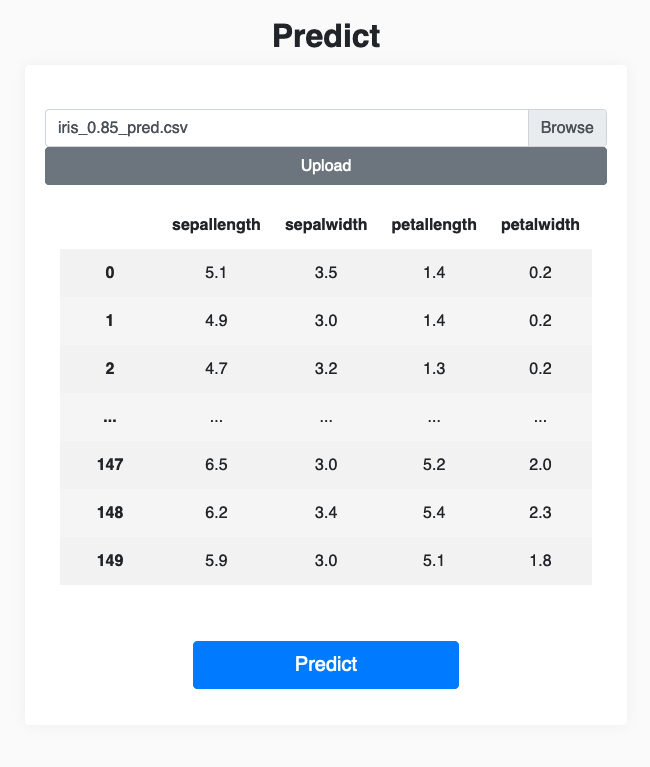
\includegraphics[scale=0.4]{../img/anexos/manual-usuario/UBUMLaaS/pre-predict}
\caption{Vista de antes de predecir.}\label{fig:pre-predict}
\end{figure}

Y posterior a la predicción se mostrarán los resultados tal y como cabría esperar, en la Figura~\ref{fig:post-predict} se muestra el ejemplo, en caso de considerar que la predicción es correcta, se mostrará en verde, en este caso todas son rojas puesto que no se garantiza su corrección.

\begin{figure}
\centering
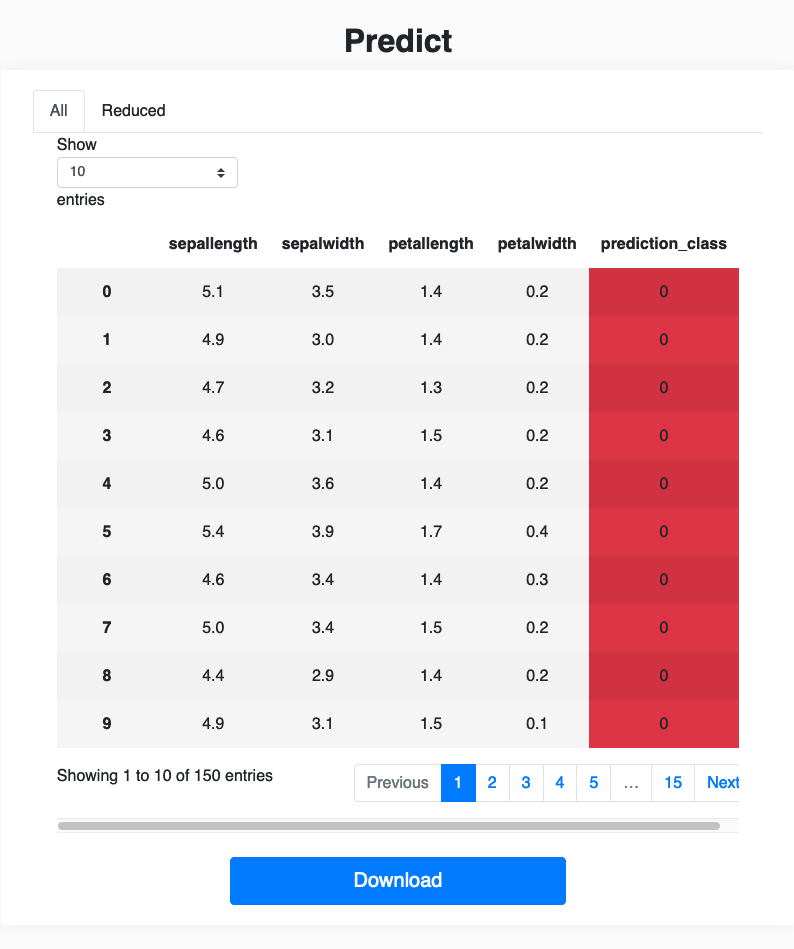
\includegraphics[scale=0.4]{../img/anexos/manual-usuario/UBUMLaaS/post-predict}
\caption{Vista de después de predecir.}\label{fig:post-predict}
\end{figure}

\FloatBarrier
\subsubsection{Estadísticas de uso}
Si se desean visualizar las estadísticas personales de uso de la aplicación, se debe acudir al perfil del usuario, el cuál es compartido con la lista de experimentos, desde la pantalla principal, Figura~\ref{fig:index-login}, (o desde cualquier otra) se deberá pulsar en la parte superior derecha sobre el botón \textit{Launched Experiments}, y se redirigirá al perfil. 

En el perfil, Figura~\ref{fig:profile}, se pulsará sobre el botón verde debajo de la foto de perfil del usuario en el lado izquierdo, el botón muestra una cadena de texto en la que se indica \textit{Statistics}. Seguidamente se abrirá una nueva \texttt{card} a la derecha, encima de todo lo que aparece, con las estadísticas del usuario. Para cerrar la vista basta con hacer \textit{click} de nuevo sobre el botón verde o sobre la cabecera de la \texttt{cart}. 

En la Figura~\ref{fig:user-stats} se muestra un ejemplo de las estadísticas de un usuario, las comentamos al detalle a continuación:
\begin{itemize}
\item Las cartas superiores son dos contadores, indican los experimentos \textbf{existentes} en la base de datos de la aplicación con identificador de usuario igual al usuario en cuestión. Y la segunda indica el número de conjunto de datos que el usuario posee en total, incluyendo los añadidos por defecto.
\item El gráfico titulado \textit{Experiments performed in the last 7 days}, tal y como la traducción referencia, muestra un gráfico con el número de experimentos que se han ejecutado por parte del usuario en los últimos 7 días, siendo el valor más a la derecha el día actual.
\item El gráfico de tipo \textit{pie} muestra el número de experimentos de cada tipo que el usuario ha ejecutado.
\item El gráfico de barras permite conocer el tiempo en total que los experimentos de un usuario han estado en ejecución en el sistema, estando agrupados por tipos de algoritmos. Se puede cambiar la escala de tiempo para una mayor comodidad de interpretación.
\end{itemize}

\imagenFlotante{../img/anexos/manual-usuario/UBUMLaaS/user-stats}{Estadísticas de usuario}{user-stats}

\FloatBarrier
\subsubsection{Modificación de datos del usuario y actualizar contraseña}
Todo usuario puede modificar sus datos personales, así como añadir una serie de datos que no son obligatorios. Para modificar los datos se realizará desde el perfil del usuario, haciendo \textit{click} en el botón amarillo en la parte inferior izquierda, con la cadena de caracteres \textit{Edit profile}.

En este momento se lanzará un modal el cual posee dos partes diferencias, modificación de datos personales, y en la parte inferior modificación de la contraseña.

Cuando se decida qué se quiere modificar, se deberá hacer \textit{click} en el \textit{checkbox} que se encuentra en la parte superior de cada formulario, lo cual habilitará la edición del mismo. Los formularios se encuentran en las Figuras~\ref{fig:edit-profile-data}~y~\ref{fig:edit-profile-passwd}, respectivamente. 

\begin{figure}
\centering
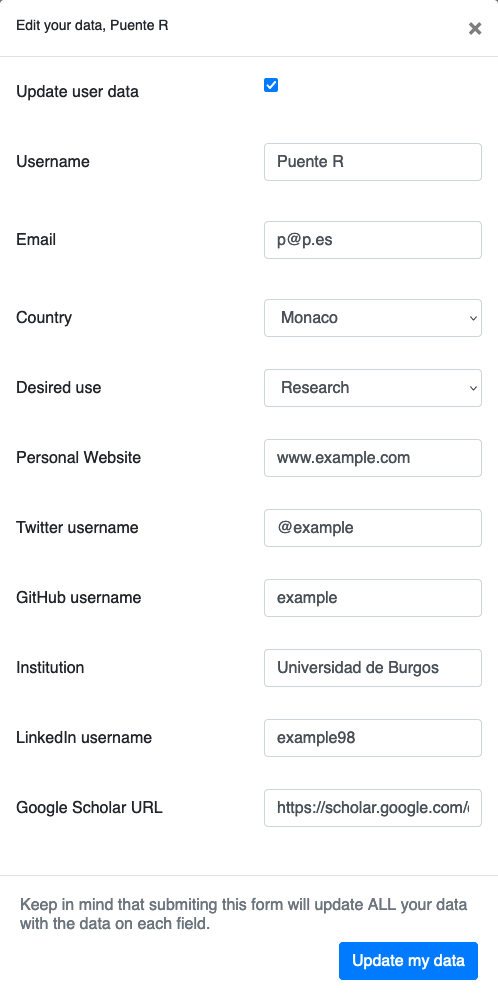
\includegraphics[scale=0.5]{../img/anexos/manual-usuario/UBUMLaaS/edit-profile-data}
\caption{Formulario de edición de los datos de un usuario.}\label{fig:edit-profile-data}
\end{figure}

\begin{figure}
\centering
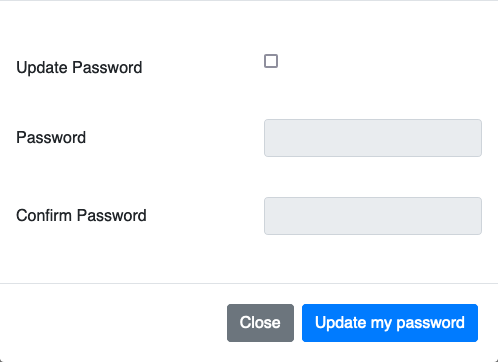
\includegraphics[scale=0.5]{../img/anexos/manual-usuario/UBUMLaaS/edit-profile-passwd}
\caption{Formulario para cambiar la contraseña de un usuario.}\label{fig:edit-profile-passwd}
\end{figure}

\FloatBarrier
\subsection{Manual del administrador}
A continuación se detallan todas las funcionalidades añadidas que posee un administrador. Un administrador es un usuario en su base, por lo tanto, todas las funcionalidades descritas en la sección anterior también hacen referencia al administrador.

\subsubsection{\texttt{NavBar} de administración}
Tal y como se aprecia en la Figura~\ref{fig:index-admin}, el administrador posee una barra de navegación lateral en toda la aplicación, permitiendo acceder a esas funcionalidades en cualquier momento desde cualquier lugar. A su vez, en la parte superior derecha posee un acceso directo a la parte de administración, el botón \textit{Administration}.

En caso de querer ocultar la barra lateral de administración, ya que no se va utilizar en ese momento, en la parte superior izquierda aparece una \texttt{X}, haciendo \textit{click} en ella se ocultará la barra lateral.

\imagenFlotante{../img/anexos/manual-usuario/UBUMLaaS/index-admin}{Vista principal de administrador.}{index-admin}

En las siguientes secciones se comentarán cada una de las opciones disponibles para los administradores.

\subsubsection{Analytics Dashboard}
Accediendo a través del botón \textit{Dashboard} en el menú lateral, se accede a la vista de analíticas del sistema, en la que aparecen tanto estadísticas de los últimos 7 días, como globales del sistema, se puede apreciar en la Figura~\ref{fig:dashboard}.

\imagenFlotante{../img/anexos/manual-usuario/UBUMLaaS/dashboard}{Vista de \textit{Analytics Dashboard}}{dashboard}

Se dispone de la siguiente información:
\begin{itemize}
\item Cartas superiores
\begin{itemize}
	\item Número total de experimentos (los modelos) que se encuentran almacenados en el sistema.
	\item Número total de conjuntos de datos distintos almacenados en el sistema.
	\item Número de usuarios registrados en el sistema.
	\item Número total del países de los cuáles los usuarios han dicho ser.
\end{itemize}
\item \textit{Experiments performed in the last 7 days}. Igual que para el usuario, pero con las estadísticas de todos los usuarios. 
\item \textit{Algorithm Type Usage Distribution}. Estadísticas globales del número de experimentos de cada tipo que se han ejecutado.
\item \textit{Algorithm Type Time Used}. Distribución del tiempo de uso (ejecución) de los diferentes tipos de algoritmos.
\item \textit{Desired Use}. Estadísticas del uso que los usuarios han indicado que le van a dar primordialmente a la aplicación.
\item \textit{Country Distribution}. Representación de la ubicación geográfica de los usuarios. Siendo representado cada país por un único punto.
\item \textit{Latests Experiments}. Últimos 10 experimentos lanzados, pueden estar \textit{In Progress}, o terminados, ya sea \textit{Finalized} o bien \textit{Error}. Mostrando la información mínima necesaria así como el usuario dueño del experimento.
\item \textit{All Time Datasets Run}. Comparativa del tiempo de ejecución de algunos conjuntos de datos en comparación con el número de veces que han sido ejecutados. Se puede modificar la escala de tiempo.
\end{itemize}

\subsubsection{Users}
Se accede a la página de administración de usuarios a través del botón \textit{Users} en la barra lateral. En este panel se pueden crear, (des)activar, dar/quitar privilegios de administración, o eliminar un usuario.

Tal y como se puede ver en la Figura~\ref{fig:users-admin}, se soporta la búsqueda por cualquiera de los campos que se visualizan, permitiendo encontrar a aquellos usuarios que interese en <<un \textit{click}>>. 

\imagenFlotante{../img/anexos/manual-usuario/UBUMLaaS/users-admin}{Vista de administración de usuarios}{users-admin}

Un usuario no puede quitarse a sí mismo privilegios de administrador, ni deactivarse la cuenta, o eliminarla, teniendo que ser otro administrador el que lo haga; de esta manera el sistema siempre tendrá como mínimo un administrador.

A su vez se soporta crear un usuario haciendo \textit{click} en el botón verde \textit{New user}. Desplegándose un formulario y se deberán de rellenar los campos de correo electrónico, nombre de usuario, país y uso que se va a hacer; las restricciones de los campos existentes deben de seguir cumpliéndose. Al usuario se le generará una contraseña y al correo electrónico llega un correo, valga la redundancia, de activación de la cuenta, pero deberá de re-establecer la contraseña como si la hubiera olvidado antes de poder iniciar sesión por primera vez.

\subsubsection{Live System Monitor}
A la monitorización del sistema en tiempo real se accede a través del botón \textit{Live System Monitor} en la barra lateral. Cuando se hace \textit{click} se redirecciona a una vista similar a la que aparece en la Figura~\ref{fig:live-monitor}. En la parte superior derecha de la página a la que se llega hay un botón para activar si se quiere que la página se auto-recargue cada 60 segundos, desde el momento en el que se hace \textit{click}.

\imagenFlotante{../img/anexos/manual-usuario/UBUMLaaS/live-monitor}{Vista de \textit{Live System Monitor}}{live-monitor}

\textbf{NOTA.} Es importante tener en cuenta que esta pantalla se ha diseñado para monitores de más de 23 pulgadas, por lo que su visualización en monitores de menor tamaño puede no ser óptima o encontrar ciertos solapamientos. En la Figura~\ref{fig:live-monitor} se aprecia la disposición correcta de todos los componentes.

La información que se muestra es la siguiente (todas las unidades que se muestran son calculadas dinámicamente, seleccionando la mayor disponible):
\begin{itemize}
\item Las cartas superiores muestran, de izquierda a derecha:
\begin{itemize}
	\item \textit{CPU Load}. La carga de la CPU porcentualmente.
	\item \textit{CPU Cores}. El número total de núcleos del sistema.
	\item \textit{Memory Load}. El uso total de la memoria en forma de gráfico.
	\item \textit{Used Memory}. El valor total de memoria en uso en el sistema.
	\item \textit{Storage in use}. Almacenamiento total del sistema en vista de gráfico.
	\item \textit{Storaged Used}. El valor total de almacenamiento en uso.
\end{itemize}
\item \textit{System Load 1/5/15}. Cada gráfico representa la carga media del sistema en los últimos 1, 5 y 15 minutos, respectivamente.
\item \textit{I/O Usage}. Interrupciones de tipo \textit{Input}/\textit{Output} de la CPU y del disco.
\item \textit{Network Usage}. Tamaño total de información transmitida y recibida en el periodo de tiempo.
\item Las cartas inferiores muestran, de izquierda a derecha:
\begin{itemize}
	\item \textit{Uptime}. Tiempo total desde que el sistema se inició. Formato: días:horas:minutos:segundos.
	\item \textit{IP Address}. Dirección IP del equipo/servidor donde se encuentra la plataforma desplegada.
	\item \textit{IP Public Address}. Dirección IP pública del sistema.
	\item \textit{IP Mask CIDR}. Máscara de subred en formato CIDR.
	\item \textit{Total Processes}. Número total de procesos que existen en el sistema en ejecución.
	\item \textit{Total Threads}. Número total de hilos en el sistema.
\end{itemize}
\end{itemize}

%%%%%%%%%%%%%%%%%%%%%%%%%%%%%%%%%%%%%%%%%%%%%%%%%%%%%%%%%%%%%%%%%%%%%%
\FloatBarrier
\section{IS-SSL}
A continuación se presenta el manual de usuario de las bibliotecas de algoritmos desarrolladas. Permitiendo a cualquier usuario comprender \texttt{IS-SSL} y poder hacer uso de las mismas.
\subsection{Requisitos de usuarios}
Los requisitos mínimos para poder hacer uso de \texttt{IS-SSL} son:
\begin{itemize}
\item Tener instalado Python 3.7+.
\item Tener instalado y configurado \texttt{PIP} o \texttt{Conda}.
\item Disponer de un editor de textos.
\item Tener instaladas las bibliotecas necesarias para su correcto funcionamiento.
\end{itemize}

\subsection{Instalación}

Por comodidad para el usuario, \texttt{IS-SSL} se ha dividido en dos bibliotecas, una formada por los algoritmos de selección de instancias, y una segunda por aquellos algoritmos de aprendizaje semi-supervisado.

El proceso de instalación de cualquiera de las dos bibliotecas es muy sencillo, siendo integrable en cualquier fichero de requerimientos, ya sea para \texttt{PIP} o \texttt{Conda}.

Las dos bibliotecas se encuentran publicadas en PyPI\footnote{\textit{Python Package Index} es un repositorio de \textit{software} para el lenguaje de programación de Python.} desde su versión 1.0, la cual fue una primea versión alpha estable con los primeros algoritmos publicados. 
La versión 3.0 es la versión estable (la final) que se ha publicado.

\imagenFlotante{../img/anexos/manual-usuario/PyPI-IS}{Vista de la biblioteca de algoritmos de selección de instancias en PyPI.}{PyPI-IS}
\imagenFlotante{../img/anexos/manual-usuario/PyPI-SSL}{Vista de la biblioteca de algoritmos de aprendizaje semi-supervisado en PyPI.}{PyPI-SSL}

Para realizar la instalación se deben seguir los siguientes pasos para cualquier LIB, LIB $\in \lbrace$ IS-DNX, SSL-DNX$\rbrace$.

\begin{enumerate}
\item Acceder a PyPi, desde~\cite{PyPI}.
\item Introducir en el campo de búsqueda <<LIB>>.
\item Seleccionar la biblioteca correspondiente de entre la lista mostrada.
\item Copiar el comando de instalación.
\item Abrir una terminal con soporte a Python y \texttt{PIP}.
\item Introducir el comando copiado.
\item En caso de que se nos pregunte si se quiere proceder con la descarga, indicar que sí con una S en caso de que esté en español, o con Y en el caso inglés/internacional.
\item Cuando finaliza la instalación, la biblioteca se encontrará lista para su uso.
\end{enumerate}

\imagenFlotante{../img/anexos/manual-usuario/PIP-IS}{Instalación de la biblioteca de selección de instancias.}{PIP-IS}
\imagenFlotante{../img/anexos/manual-usuario/PIP-SSL}{Instalación de la biblioteca de semi-supervisado.}{PIP-SSL}


\subsection{Manual del usuario}

A continuación se documentan las funcionalidades de las bibliotecas, desde su importación, a uso y especificación de los diferentes parámetros de entrada y salida esperados. A modo de resumen se puede destacar que todos los algoritmos siguen la misma estructura interna luego el aprendizaje y familizarización es relativamente rápido.

\subsubsection{Biblioteca de algoritmos de selección de instancias}
\textbf{Importar}

Para poder trabajar con los algoritmos de selección de instancias se deben de importar en el fichero en el que se quieran utilizar. Para ello se importan como cualquier otro paquete de Python, supongamos que queremos utilizar el algoritmo ENN, lo importaremos de la siguiente manera:

\texttt{from InstanceSelectionDNX import ENN} 

De esta forma podemos sustituir ENN por el algoritmo que deseemos de entre los disponibles y tenerlo a nuestra disposición para su uso.

Todos los algoritmos están codificados como \texttt{class} por lo tanto se debe de instanciar antes de poder hacer uso del mismo. 

\textbf{Uso}

Como se ha comentado al comienzo, todos los algoritmos poseen la misma estructura. Todos ellos poseen el método \texttt{filter} de tal manera que una vez se haya instanciado se podrá llamar al método y se obtendrá como resultado el conjunto de datos reducido.

Todos los algoritmos en su instanciación reciben aquellos parámetros que son necesarios para la configuración y su uso posterior, mientras que cuando se realiza el filtrado únicamente reciben el conjunto de datos dividido, por un lado los atributos y por otro lado la clase.

Tanto las entradas como las salidas deben ser objetos de tipo \texttt{DataFrame} de \texttt{Pandas}.

\begin{lstlisting}[language=python, caption={Ejemplo de uso de ENN}]]
from InstanceSelectionDNX import ENN
import pandas as pd

data = pd.DataFrame([[1, 2, 3, 4],
        [4, 3, 2, 1],
        [1, 2, 4, 3],
        [2, 1, 3, 4]])
target = pd.DataFrame([0, 0, 1, 1])

model = ENN(nearest_neighbors=3, power_parameter=2)

data_red, label_red = model.filter(data, target)
\end{lstlisting}

\subsubsection{Biblioteca de algoritmos de aprendizaje semi-supervisado}
\textbf{Importar}

De manera análoga a la otra biblioteca, importaremos el paquete y seleccionaremos cuál es el algoritmo que se desea utilizar, por ejemplo:

\texttt{from SemiSupervisedLearningDNX import TriTraining}

Pudiendo sustituir TriTraining por el algoritmo deseado.

Todos los algoritmos están codificados como \texttt{class} por lo tanto se debe de instanciar antes de poder hacer uso del mismo. 

\textbf{Uso}

Los algoritmos siguen la misma estructura interna que los propios de \texttt{Scikit-Learn}, por lo que una vez instanciados (con sus respectivos parámetros de configuración) bastará con llamar al método \texttt{fit} de cada uno de ellos, así como para predecir al método correspondiente, denominado \texttt{predict}.

\begin{itemize}
\item \textbf{\texttt{fit}:} recibe como argumentos dos parámetros, las instancias y las etiquetas o clases, siendo -1 aquellas que se desconozcan y se quieran utilizar para entrenar el algoritmo.
\item \textbf{\texttt{predict}:} recibe únicamente las instancias que se quieren etiquetar. Devuelve estas instancias etiquetadas.
\end{itemize}

Todas las entradas como las salidas deben ser objetos de tipo \texttt{DataFrame} de \texttt{Pandas}.

\begin{lstlisting}[language=Python, caption={Ejemplo de uso de IS-SSL}, label={lst:ejemplossl}]
from SemiSupervisedLearningDNX import TriTraining
from sklearn.naive_bayes import GaussianNB
from sklearn.neighbors import KNeighborsClassifier
from sklearn.datasets import load_iris
	
model = TriTraining(
	random_state = 42,
	c1 = GaussianNB, c1_params = None,
	c2 = KNeighborsClassifier, c2_params = {n_neighbors: 2}
)
	
iris = load_iris()
X = iris['data']
y = iris['target']

X = pd.DataFrame(X), y = pd.DataFrame(y)
	
val = [True if i % 2 == 0 else False for i in range(len(y))]
y.loc[val] = -1

X, X_test, y, y_test = train_test_split(X.to_numpy(), y.to_numpy())

X = pd.DataFrame(X), y = pd.DataFrame(y)

model.fit(X, y)
y_pred = model.predict(X_test)
	
\end{lstlisting}
\vfill
\subsubsection{Ejemplo de uso combinado de ambas bibliotecas}
\begin{lstlisting}[language=Python, caption={Ejemplo de uso de IS-SSL}, label={lst:ejemplo}]
from SemiSupervisedLearningDNX import TriTraining
from InstanceSelectionDNX import ENN
from sklearn.naive_bayes import GaussianNB
from sklearn.neighbors import KNeighborsClassifier
from sklearn.tree import DecisionTreeClassifier
from sklearn.datasets import load_iris
	
if __name__ == "__main__":
	model = TriTraining(
		random_state = 42,
		c1 = GaussianNB, c1_params = None,
		c2 = KNeighborsClassifier, c2_params = {n_neighbors: 2},
		c3 = DecisionTreeClassifier, c3_params = None	
	)
	filter_model = ENN(nearest_neighbors = 5, power_parameter = 2)
	
	iris = load_iris()
	X = iris['data']
	y = iris['target']

	X = pd.DataFrame(X)
	y = pd.DataFrame(y)
	X, y = filter_model.filter(X, y)

	val = [True if i % 2 == 0 else False for i in range(len(y))]
	y[val] = -1

	X, X_test, y, y_test = train_test_split(X.to_numpy(), y.to_numpy())

	X = pd.DataFrame(X)
	y = pd.DataFrame(y)

	model.fit(X, y)
	y_pred = model.predict(X_test)
	print(accuracy_score(y_true=y_test, y_pred=y_pred))
	
\end{lstlisting}